\documentclass{beamer}

\usepackage{calc}
\usepackage{ifthen}

% Pie chart
% Author: Robert Vollmert
\newcounter{temp}


% calculate the anchor of the external label
\newcommand{\angledir}[1]{
  \setcounter{temp}{#1}

  \ifthenelse{\thetemp < 0}{\addtocounter{temp}{360}}{}
  \ifthenelse{\thetemp > 360}{\addtocounter{temp}{-360}}{}

  \ifthenelse{\thetemp < 11}{\def\piedir{right}}{
  \ifthenelse{\thetemp < 80}{\def\piedir{above right}}{
  \ifthenelse{\thetemp < 101}{\def\piedir{above}}{
  \ifthenelse{\thetemp < 170}{\def\piedir{above left}}{
  \ifthenelse{\thetemp < 191}{\def\piedir{left}}{
  \ifthenelse{\thetemp < 260}{\def\piedir{below left}}{
  \ifthenelse{\thetemp < 281}{\def\piedir{below}}{
  \ifthenelse{\thetemp < 350}{\def\piedir{below right}}{
    right}}}}}}}}%
}

% calculate the position of the internal label
\newcommand{\calcpiedist}[1]{%
  \ifthenelse{#1 > 120}{\def\piedist{0.50}}{
  \ifthenelse{#1 < 10}{\def\piedist{0.80}}{
    \setcounter{temp}{(80 * (120-#1) + 50 * (#1-10))/110}
    \def\piedist{0.\thetemp}}}
}

% draw a slice of a pie chart
% The diffI and diffII counters are just a quick hack for making the
% code compatible with PGF 1.18
% The code should be rewritten to utilize the new math engine.
\newcounter{diffI}
\newcounter{diffII}
\newcommand{\slice}[5]{%
  \setcounter{temp}{(#1+#2)/2}
  \setcounter{diffI}{#1-\thetemp}
  \setcounter{diffII}{#2-\thetemp}
  \begin{scope}[rotate=\thetemp]
  %\pgfmathparse{#1-\thetemp}
    \draw[fill=#5,join=round]
                                (0,0)
                             -- (\thediffI:1)
                             arc (\thediffI:\thediffII:1)
                             -- cycle;
    \angledir{\thetemp}
    \node [\piedir] at (1,0) {#4};
    \setcounter{temp}{#2-#1}
    \calcpiedist{\thetemp}
    \node at (\piedist,0) {#3};

  \end{scope}
}



\mode<presentation>
{
	\usepackage{StyleFiles/Rome}
	\setbeamercovered{transparent}
}

\mode<handout>
{
	\usepackage{pgfpages}
	\pgfpagesuselayout{2 on 1}[a4paper,border shrink=5mm]
	\nofiles
}

\usepackage{pgfplots}
\usepackage{tikz}
\usepackage{pgf}
\usepackage{multimedia}
\usepackage{hyperref}
\usepackage{listings}
\usepackage[english]{babel}
\usepackage[latin1]{inputenc}
\usepackage{mathptmx}
\usepackage{helvet}
\usepackage[T1]{fontenc}

\title[Multi-Clustered PF for DDF]{Multi-Clustered Particle Filter for Distributed Data Fusion}

\subtitle{}

\author[Fabio Previtali]{\textbf{Fabio Previtali}}

\date[19/07/2011]{Master Thesis - Rome, Italy}

\begin{document}

\begin{frame}[plain]
	\titlepage
\end{frame}

\section{Introduction to Distributed Data Fusion}

\begin{frame}
	\frametitle{Multi-Agent Multi-Object Tracking (MAMOT)}
	\framesubtitle{A brief overview}
	
	\begin{columns}
		\column{.7\textwidth}
		\centering
		
		\begin{block}{Object Tracking}
			Detect objects and follow their trajectories
		\end{block}
		
		\begin{block}{MAMOT}
			A team of agents estimate the object trajectories using sensors with a limited field-of-view
		\end{block}
		
		\begin{itemize}
			\item distributed environment (network connected agents)
			\item best-effort communication channel
		\end{itemize}
		
		\column{.28\textwidth}
		\centering
		
		\begin{tikzpicture}
			\node at (0,0) [draw=black,ultra thick,inner sep=0pt]  {\includegraphics[width=3cm]{Figures/Player.png}};
		\end{tikzpicture}
	\end{columns}
\end{frame}

\begin{frame}
	\frametitle{Issues on DDF}
	\framesubtitle{The Data Association problem}
	
	\begin{columns}[T]
		\column{.55\textwidth}
		
		\begin{itemize}
			\only<1>{\item In MAMOT, the pool of gathered parameters are used to compute the global estimation}
			\only<1>{\item Using a Particle Filter, one of the main problem that arises is how to avoid poor estimation
						   quality}
			\only<1>{\vspace{3.42cm}}
			\only<2->{\item The weight of particles is evaluated using the received parameters}
			\only<3->{\vspace{1.5cm}\item[1] Using all parameters influences the whole distribution}
			\only<4-5>{\vspace{1.1cm}}
			\only<6>{\vspace{0.9cm}}
			\only<4>{\item[2] We can assign better weights by use clustering before weighting}
			\only<5>{\item[2] The parameters are associated to the clusters}
			\only<6>{\item[2] The weights of particles in a cluster is given by the parameters associated to it}
		\end{itemize}
		
		\column{.45\textwidth}
		\centering
		
		\begin{tikzpicture}
			\only<1>
			{
				\node at (0,0) [draw=white,thick,inner sep=0pt]  {\includegraphics[width=5cm]{Figures/MamotDDF.pdf}};
			}
			\only<2->
			{
				\node at (-1.3,0) [draw=white,thick,inner sep=0pt]  {\includegraphics[width=2.5cm]{Figures/Issue0.pdf}};
				\node at (1.3,0) [draw=white,thick,inner sep=0pt]  {\includegraphics[width=2.5cm]{Figures/Issue0Bis.pdf}};
				\node at (0,-1) [inner sep=0pt]  {\includegraphics[width=5cm]{Figures/Parentheses.pdf}};
				\node at (0,-2.5) [draw=white,thick,inner sep=0pt]  {\includegraphics[width=4cm]{Figures/IssueBlank.pdf}};
				\node at (0,-4.8) [draw=white,thick,inner sep=0pt]  {\includegraphics[width=4cm]{Figures/IssueBlank.pdf}};
			}
			\only<3->
			{
				\node at (0,-2.5) [draw=white,thick,inner sep=0pt]  {\includegraphics[width=4cm]{Figures/Issue1.pdf}};
				\node at (0,-4.8) [draw=white,thick,inner sep=0pt]  {\includegraphics[width=4cm]{Figures/IssueBlank.pdf}};
			}
			\only<4>
			{
				\node at (0,-4.8) [draw=white,thick,inner sep=0pt]  {\includegraphics[width=4cm]{Figures/Issue2.pdf}};
			}
			\only<5>
			{
				\node at (0,-4.8) [draw=white,thick,inner sep=0pt]  {\includegraphics[width=4cm]{Figures/Issue2Bis.pdf}};
			}
			\only<6>
			{
				\node at (0,-4.8) [draw=white,thick,inner sep=0pt]  {\includegraphics[width=4cm]{Figures/Issue2Ter.pdf}};
			}
		\end{tikzpicture}
	\end{columns}
\end{frame}

\section{Multi-Clustered Particle Filtering}

\begin{frame}
	\frametitle{Multi-Clustering Particle Filtering}
		\begin{columns}
			\column[T]{.5\textwidth}
			
			\begin{enumerate}
				\item<2-> system state evolution
				\item<3-> local system state estimation
				\item<4-> gathering global information
				\item<6-> clusterisation
				\item<7-> data association
				\item<8-> global estimation
			\end{enumerate}
			
			\column[T]{.5\textwidth}
			\centering
			\includegraphics[width=5.5cm]<1>{Figures/Mamot0.pdf}
			\includegraphics[width=5.5cm]<2>{Figures/Mamot1.pdf}
			\includegraphics[width=5.5cm]<3>{Figures/Mamot2.pdf}
			\includegraphics[width=5.5cm]<4>{Figures/Mamot3.pdf}
			\includegraphics[width=5.5cm]<5>{Figures/Mamot3Bis.pdf}
			\includegraphics[width=5.5cm]<6>{Figures/Mamot4.pdf}
			\includegraphics[width=5.5cm]<7>{Figures/Mamot5.pdf}
			\includegraphics[width=5.5cm]<8>{Figures/Mamot6.pdf}
		\end{columns}
\end{frame}

\begin{frame}
	\frametitle{Clustering Correlation}
	\begin{columns}[T]
		\column{.5\textwidth}
		\centering
		\begin{itemize}
			\item Particles' clusterisation in order to detect targets \\
				  $ \leadsto $ approximatively each cluster corresponds to an estimated target
			\item Dynamic threshold function used to separate the clusters
			\item It depends on:
			
			\begin{itemize}
				\item complexity of world
				\item expected number of targets
				\item field-of-view of agent's sensors
			\end{itemize}
		\end{itemize}
		
		\column{.6\textwidth}
		\centering
		
		\begin{tikzpicture}
			\node at (0,0) [draw=black,thick,inner sep=0pt]{\includegraphics[width=2.5cm]{Figures/Mamot4.pdf}};
		\end{tikzpicture}
		\begin{tikzpicture}
			\node at (0,0) [draw=black,thick,inner sep=0pt]{\includegraphics[width=2.5cm]{Figures/Mamot5.pdf}};
		\end{tikzpicture}\\
		\vspace{0.2cm}
		\begin{tikzpicture}
			\node at (0,0) [draw=black,thick,inner sep=0pt]{\includegraphics[width=3cm]{Figures/Mamot6.pdf}};
		\end{tikzpicture}
	\end{columns}
\end{frame}

\section{Experimental Results}

\begin{frame}
	\frametitle{Performance Evaluation}
	\begin{itemize}
		\item The effectiveness of our approach compared to Multi-Filter Particle Filtering approach as proposed in
			  [Okuma et al, 2004]\footnote{K. Okuma, A. Taleghani, N. d. Freitas, J. J. Little, and D. G. Lowe, \\
			  \hspace{0.6cm}\emph{``A boosted particle filter: Multitarget detection and tracking''}, 2004} and 
			  [Wu et al, 2008]\footnote{Y. Wu, X. Tong, Y. Zhang, and H. Lu,\\\hspace{0.6cm}\emph{``Boosted
			  interactively distributed particle filter for automatic multi-object\\\hspace{0.6cm}tracking''}, 2008}
		\item Several metrics are used, to cover the majors interesting aspects of the DDFS
		\item Multiple maps are used to increase reliability of results
	\end{itemize}
\end{frame}

\begin{frame}
	\frametitle{Simulation Setup}
	\begin{columns}[T]
		\column{.6\textwidth}
		
		\begin{itemize}
			\item Player/Stage simulator
				\begin{itemize}
					\item 4 different maps
					\item each map has an area $\sim 600 m^2$
					\item $90\%$ of each map is empty space
				\end{itemize}
				\vspace{0.4cm}
			\item Agent sensor field of view
				\begin{itemize}
					\item $\rho = 10m$
					\item $\theta = 62^{\circ}$
					\item $\leadsto$ area = $\frac{\rho^2\theta}{2} \sim 54 \mathrm{m}^2$
				\end{itemize}
				\vspace{0.4cm}
			\item Operational assumptions
				\begin{itemize}
					\item Random paths
					\item Synchronized agents
					\item Fully distributed
				\end{itemize}
		\end{itemize}
		
		\column{.5\textwidth}
		\centering
		\begin{tikzpicture}[map/.style={draw=black,ultra thick,inner sep=0pt}]
			\node at (-1.1,0.8) [map] {\includegraphics[height=1.2cm,width=1.8cm]{Maps/Edmonton}};
			\node at (-1.3,-0.1) [map] {\includegraphics[height=1.2cm,width=1.8cm]{Maps/Longwood}};
			\node at (0.3,-0.4) [map] {\includegraphics[height=1.2cm,width=1.8cm]{Maps/Mexico}};
			\node at (0.2,0.6) [map,draw=red!70!black] {\includegraphics[height=1.4cm,width=2.1cm]{Maps/Lasermaze}};
		\end{tikzpicture} \\
		\vspace{0.1cm}
		\begin{tikzpicture}
			\node at (0,0) [draw=black,ultra thick,inner sep=0pt]  {\includegraphics[height=1.8cm]{Figures/Agent.pdf}};
		\end{tikzpicture} \\
		\vspace{0.2cm}
		\begin{tikzpicture}
			\node at (0,0) [draw=black,ultra thick,inner sep=0pt]  {\includegraphics[width=3cm]{Figures/Stage.png}};
		\end{tikzpicture}
	\end{columns}
\end{frame}

\begin{frame}
	\frametitle{Simulation Setup - cont'd}
	\framesubtitle{Artificial noise}
	\begin{columns}[T]
		\column{.5\textwidth}
		
		\begin{itemize}
			\item Gaussian noise
				\begin{itemize}
					\item added to measurements at every iteration
				\end{itemize}
			\vspace{0.5cm}
			\item False positive
				\begin{itemize}
					\item the perception is changed with probability $ p $
				\end{itemize}
			\vspace{0.5cm}
			\item True negative
				\begin{itemize}
					\item a perception is ignored with probability $ q $
				\end{itemize}
		\end{itemize}
		
		\column{.5\textwidth}
		\centering
		\includegraphics[width=2.5cm]{Figures/ErrorGauss.pdf} \\
		\vspace{0.1cm}
		\includegraphics[width=2.5cm]{Figures/ErrorFalse.pdf} \\
		\vspace{0.1cm}
		\includegraphics[width=2.5cm]{Figures/ErrorTrue.pdf}
	\end{columns}
\end{frame}

\pgfplotsset
{
	mcpc/.style={color=green!80!black,mark=triangle,draw,dashed,thick},
	mcgauss/.style={color=red!80!black,mark=square,draw,densely dotted,thick},
	mfpc/.style={color=blue!80!white,mark=o,draw,dashed,thick},
	mfgauss/.style={color=magenta,mark=star,draw,densely dotted,thick},
	axis/.style={color=black!90},
	grid/.style={very thin, dashed, color=gray, step=0.2cm},
	ymin=0,
	xmin=0.17,
	xmax=1.02,
	tick label style={font=\tiny},
	y tick label style={rotate=90},
	width=6.5cm,
	height=3.3cm,
	x label style={inner sep=-2pt},
	axis y line*=right,
	figtop/.style={xtick=\empty},
	figmiddle/.style={yshift=-50,axis x line*=bottom,xtick=\empty},
	figbottomT/.style={yshift=-100,axis x line*=bottom,xlabel=\scriptsize{$\Delta_{\mathcal{A}}$},},
	legend style={font=\tiny,baseline}
}

\tikzset
{
	smooth,
	mark options={solid,thick}
}

\begin{frame}
	\frametitle{Evaluation Metrics}
		\begin{itemize}
			\item Root Mean Squared Error
				\begin{eqnarray*}
					\delta_r = \min_{s = 1}^{\mathcal{S}} \{\|s,r\|\},
					RMSE = \sqrt{\frac{\sum_{r = 1}^{\mathcal{R}} \delta_r}{R}}.
				\end{eqnarray*}
				
				\item Execution Time
					\begin{itemize}
						\item fraction of time used by MAS algorithm
					\end{itemize}
				\item Detection rate
					\begin{displaymath}
						DR =
						\left\{
							\begin{array}{rl}
								100.0 & \mbox{if } R \leq S \\
								\{1.0 - [(R - S) / R]\} * 100.0 & \mbox{otherwise}.
							\end{array}
						\right.
					\end{displaymath}
				\item False detection rate
					\begin{displaymath}
						FR =
						\left\{
							\begin{array}{rl}
								0.0 & \mbox{if } R \geq S \\
								\{1.0 - [(S - R) / S]\} * 100.0 & \mbox{otherwise}.
							\end{array}
						\right.
					\end{displaymath}
		\end{itemize}
\end{frame}

\begin{frame}
	\frametitle{Results}
	\framesubtitle{Root Mean Squared Error}
	\begin{columns}
		\column{.5\textwidth}
		
		\begin{itemize}
			\item Our approach overtakes the Multi-Filter in terms of performance
			\item Mean error is significantly smaller
		\end{itemize}
		
		\column{.5\textwidth}
		\centering
	\begin{center}
		\begin{tikzpicture}
			\def\respath{Results/Edmonton/RMSE/Edmonton}
			\foreach \res/\fig/\leg in {0.2/figtop/legend columns=-1,0.6/figmiddle/legend columns=-1,1.0/figbottomT/{legend columns=-1,legend entries={MC-PC,MC-G,MF-PF,MF-G},legend to name=named}}
			{
				\draw node[rotate=90] at (-0.4,-4.3*\res+2) {\scriptsize{$\res$}};
				\begin{axis}[ymax=14,\fig,\leg]
					\addplot[mcpc] file {\respath.MC-PC.\res.dat};
					\addplot[mcgauss] file {\respath.MC-G.\res.dat};
					\addplot[mfpc] file {\respath.MF-PC.\res.dat};
					\addplot[mfgauss] file {\respath.MF-G.\res.dat};
					\addplot[axis,color=black] coordinates {(0.17,0) (0.17,50)};
				\end{axis}
			}
			\draw node[rotate=90] at (-0.4,-3.2) {\scriptsize{$\Delta_{\mathcal{T}}$}};
		\end{tikzpicture} \\
		
		\vspace{0.1cm}
		
		\ref{named}
	\end{center}
	\end{columns}
\end{frame}

\begin{frame}
	\frametitle{Results - cont'd}
	\framesubtitle{Execution Time}
	\begin{columns}
		\column{.5\textwidth}
		
		\begin{itemize}
			\item Clustering phase lasts longer and it is present just in our approach
			\item Both algorithms are very fast
			\item Particle Clouds approach runs faster than Gaussian one
		\end{itemize}
		
		\column{.5\textwidth}
		\centering
		
		\begin{tikzpicture}
			\def\respath{Results/Edmonton/ET/Edmonton.ET}
			\foreach \res/\fig in {0.2/figtop,0.6/figmiddle,1.0/figbottomT}
			{
				\draw node[rotate=90] at (-0.4,-4.3*\res+2) {\scriptsize{$\res $}};
				\begin{axis}[ymax=50,ytick={25,50},\fig,yticklabels={25\%,50\%}]
					\addplot[mcpc] file {\respath.MC-PC.\res.dat};
					\addplot[mcgauss] file {\respath.MC-G.\res.dat};
					\addplot[mfpc] file {\respath.MF-PC.\res.dat};
					\addplot[mfgauss] file {\respath.MF-G.\res.dat};
					\addplot[grid] coordinates {(0.17,25) (1.02,25)};
					\addplot[axis,color=black] coordinates {(0.17,0) (0.17,50)};
				\end{axis}
				\draw node[rotate=90] at (-0.4,-3.2) {\scriptsize{$\Delta_{\mathcal{T}}$}};
			}
		\end{tikzpicture} \\
		
		\vspace{0.1cm}
		
		\ref{named}
	\end{columns}
\end{frame}

\begin{frame}
	\frametitle{Results - cont'd}
	\framesubtitle{Detection Rate}
	\begin{columns}
		\column{.5\textwidth}
		
		\begin{itemize}
			\item Multi-Filter is more accurate in detecting targets
				\begin{itemize}
					\item This can be explained considering that MF is more reactive on generating filters to follow new
						  targets
				\end{itemize}
			\item Our approach, instead, in case of targets close to each other fails on creating separated cluster
		\end{itemize}
		
		\column{.5\textwidth}
		\centering
		
		\begin{tikzpicture}
			\def\respath{Results/Edmonton/DR/Edmonton.DR}
			\foreach \res/\fig in {0.2/figtop,0.6/figmiddle,1.0/figbottomT}
			{
				\draw node[rotate=90] at (-0.4,-4.3*\res+2) {\scriptsize{$\res $}};
				\begin{axis}[ymax=100,ytick={50,100},\fig,yticklabels={50\%,100\%}]
					\addplot[mcpc] file {\respath.MC-PC.\res.dat};
					\addplot[mcgauss] file {\respath.MC-G.\res.dat};
					\addplot[mfpc] file {\respath.MF-PC.\res.dat};
					\addplot[mfgauss] file {\respath.MF-G.\res.dat};
					\addplot[grid] coordinates {(0.17,50) (1.02,50)};
					\addplot[axis,color=black] coordinates {(0.17,0) (0.17,100)};
				\end{axis}
				\draw node[rotate=90] at (-0.4,-3.2) {\scriptsize{$\Delta_{\mathcal{T}}$}};
			}
		\end{tikzpicture} \\
		
		\vspace{0.1cm}
		
		\ref{named}
	\end{columns}
\end{frame}

\begin{frame}
	\frametitle{Results - cont'd}
	\framesubtitle{False Positive Detection Rate}
	\begin{columns}
		\column{.5\textwidth}
		
		\begin{itemize}
			\item Our Multi-Clustered approach has a negligible error in false targets detection
			\item $ \leadsto $ this is an important results towards real-world applications
		\end{itemize}
		
		\column{.5\textwidth}
		\centering
		
		\begin{tikzpicture}
			\def\respath{Results/Edmonton/FR/Edmonton.FR}
			\foreach \res/\fig in {0.2/figtop,0.6/figmiddle,1.0/figbottomT}
			{
				\draw node[rotate=90] at (-0.4,-4.3*\res+2) {\scriptsize{$\res $}};
				\begin{axis}[ymax=50,ytick={25,50},\fig,yticklabels={25\%,50\%}]
					\addplot[mcpc] file {\respath.MC-PC.\res.dat};
					\addplot[mcgauss] file {\respath.MC-G.\res.dat};
					\addplot[mfpc] file {\respath.MF-PC.\res.dat};
					\addplot[mfgauss] file {\respath.MF-G.\res.dat};
					\addplot[grid] coordinates {(0.17,25) (1.02,25)};
					\addplot[axis,color=black] coordinates {(0.17,0) (0.17,50)};
				\end{axis}
				\draw node[rotate=90] at (-0.4,-3.2) {\scriptsize{$\Delta_{\mathcal{T}}$}};
			}
		\end{tikzpicture} \\
		
		\vspace{0.1cm}
		
		\ref{named}
	\end{columns}
\end{frame}

\section{Conclusions}

\begin{frame}
	\frametitle{Conclusions}
		\begin{itemize}
			\item Global error estimation is reduced using Multi-Clustered approach respect to Multi-Filter
			\item Average errors are comparable using all maps
			\item The proposed approach is more robust to false perceptions respect to Multi-Filter approach
			\item The Multi-Clustered Particle Filter algorithm is suitable to be used in dynamic environments due to its
				  characteristics of \emph{reliability} and \emph{robustness}
		\end{itemize}
\end{frame}

\begin{frame}
	\frametitle{Future Works}
	\begin{columns}[T]
		\column{.65\textwidth}
		
		\begin{itemize}
			\item Improving clustering phase
			\item Use systematic noise
			\item Test the architecture in a more decision-driven scenario (like Prey-Predator model)
			\item Evaluate the impact of the algorithm on real-world environment
		\end{itemize}
		
		\column{.35\textwidth}
		\centering
		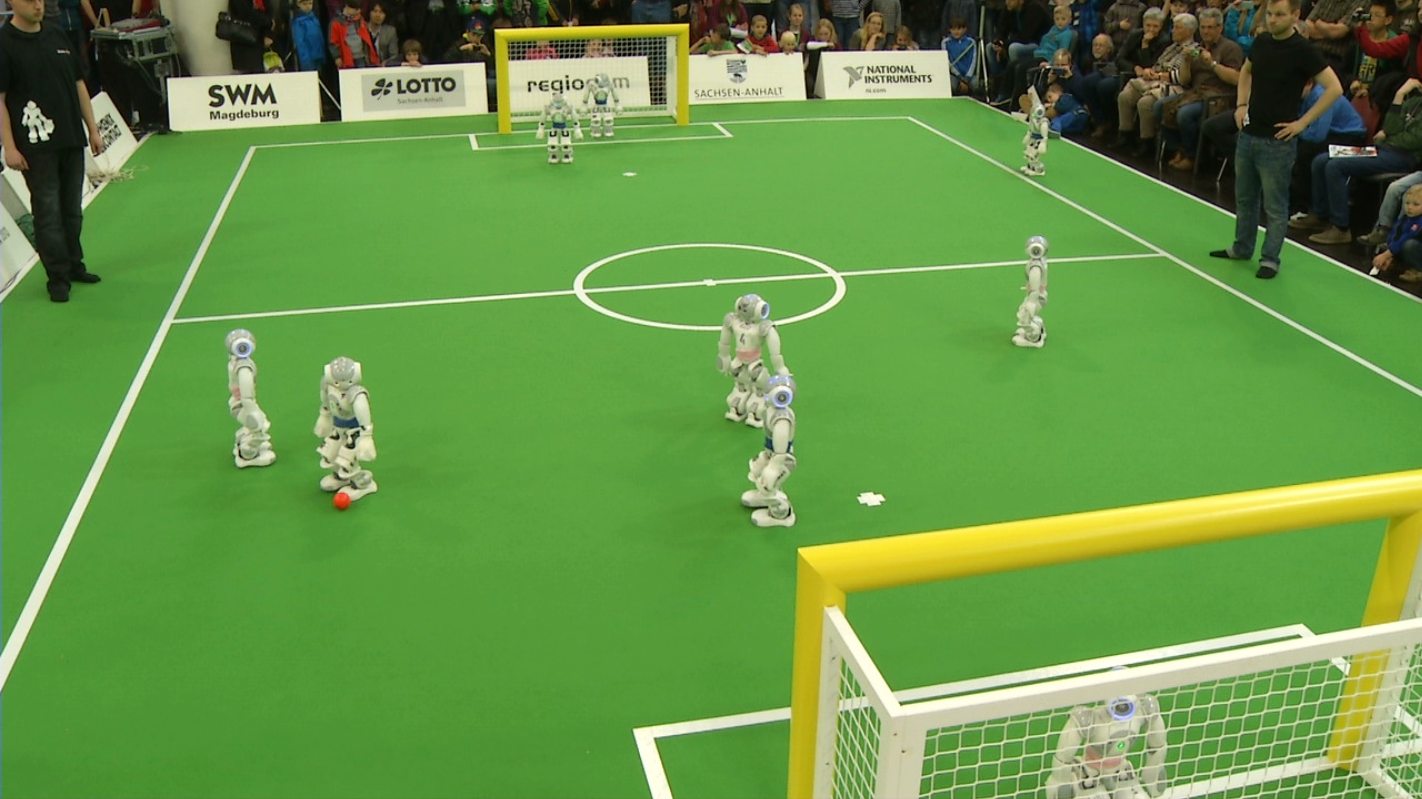
\includegraphics[width=3cm]{Figures/Nao.jpg}
	\end{columns}
\end{frame}

\begin{frame}
	\frametitle{That's all!}
	\begin{center}
		\Large{\textbf{Thank you for your attention}}
	\end{center}
\end{frame}


\end{document}
